\chapter{\en{Virtual Environment Set up}}

\section{\en{GNS3 Installation}}

Το \en{GNS3} είναι ένα λογισμικό που χρησιμοποιείται για την εξομοίωση, τη διαμόρφωση και τη δοκιμή ενός περιβάλλοντος δικτύου. Είναι
είναι ένα ελεύθερο λογισμικό ανοικτού κώδικα και μπορείτε να το κατεβάσετε από τον επίσημο δικτυακό τόπο 
\en{https://www.gns3.com/} .Το \en{GNS3} αποτελείται από δύο στοιχεία. Το ολοκληρωμένο λογισμικό (\en{GUI}) το οποίο είναι ένα γραφικό 
διεπαφή χρήστη και την εικονική μηχανή (\en{VM}), η οποία είναι ένας διακομιστής που εκτελείται σε εικονικό περιβάλλον και παρέχει καλύτερο μέγεθος τοπολογίας και υποστήριξη συσκευών.
Η εγκατάσταση είναι απλή και θα πρέπει να χρησιμοποιούνται οι προεπιλεγμένες επιλογές.

Για να γίνει σωστά η εγκατάσταση θα πρέπει το \en{software version} του \en{GNS3} να είναι το ίδιο με το
\en{software version} του \en{GNS3 VM}. Όταν λοιπόν γίνει η εγκατάσταση και ανοίγουμε το \en{GNS3 GUI}
αυτή η ενέργεια θα κάνει \en{trigger} το \en{booting} του \en{GNS3 VM}
Μόλις γίνει η εγκατάσταση μπορεί να ανοίξει η εφαρμογή και να κάνουμε \en{import cisco IOS images}. Στην παρακάτω
εικόνα μπορούμε να δούμε τι γίνεται όταν ανοίγουμε το \en{GNS3}. 

\begin{figure}[htb]
	\centering
	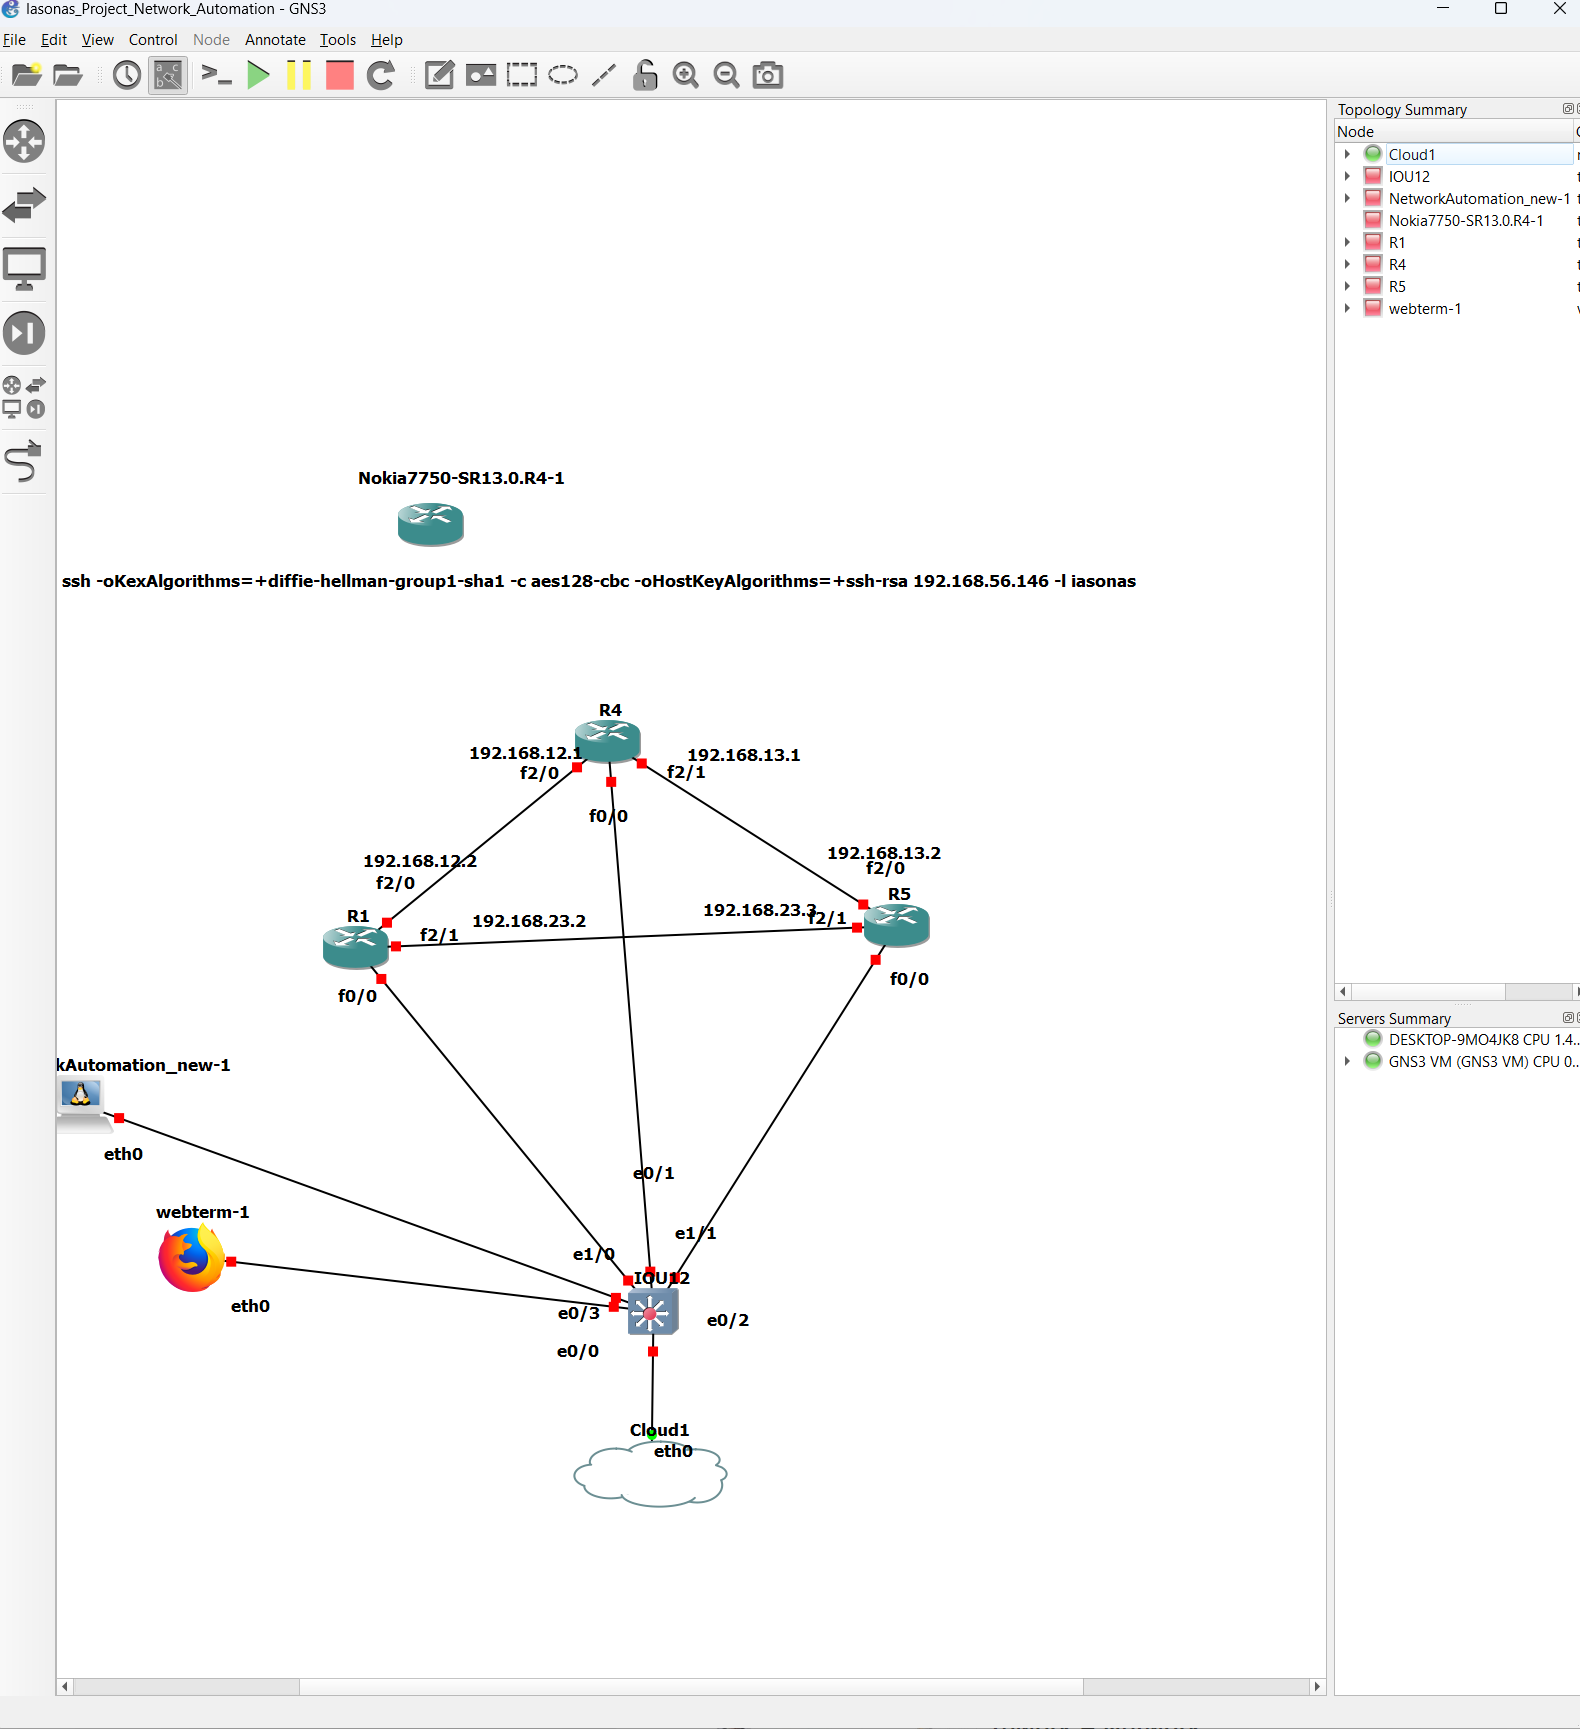
\includegraphics[width=0.7\textwidth]{graphics/gns3_homepage.png}
	\caption{\en{GNS3 homepage} }
\end{figure}

Προκειμένου να μπορέσει να επικοινωνήσει το \en{PC} μας στο τοπικό δίκτυο με το \en{GNS3 VM} στο τοπικό δίκτυο
θα πρέπει να γίνουν κάποιες ρυθμίσεις τόσο στο \en{GNS3 VM} όσο και στις συσκευές της \en{Cisco}

Στις συσκευές της \en{Cisco} θα πρέπει να γίνει η παρακάτω παραμετροποίηση όπως εμφανίζεται στις εικόνες 4.1,4.2,4.3.

\begin{figure}[htb]
	\centering
	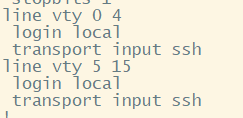
\includegraphics[width=0.7\textwidth]{graphics/cisco_ssh_config.png}
	\caption{\en{Cisco ssh config} }
\end{figure}

\begin{figure}[htb]
	\centering
	
\includegraphics[width=0.7\textwidth]{graphics/dhcp_cisco_config.png}
	\caption{\en{Cisco dhcp config} }
\end{figure}


Μέχρι αυτή τη στιγμή έχουμε παραμετροποιήσει τις συσκευές με τέτοιο τρόπο ώστε να δέχονται
απομακρυσμένη σύνδεση. Τώρα θα εξηγήσουμε πως μπορούμε να φτιάξουμε την εποικοινωνία μεταξύ εικονικών
μηχανών της \en{Cisco} και του τοπικού μας υπολογιστή. Η λογική είναι ότι η συσκευή \en{Cloud}
θα μας επιτρέψει να φτιάξουμε τη σύνδεση αυτή. Η εικόνα 4.4 μας παρουσιάζει σε ανώτερο επίπεδο τη λογική αυτή σύνδεση.

\begin{figure}[htb]
	\centering
	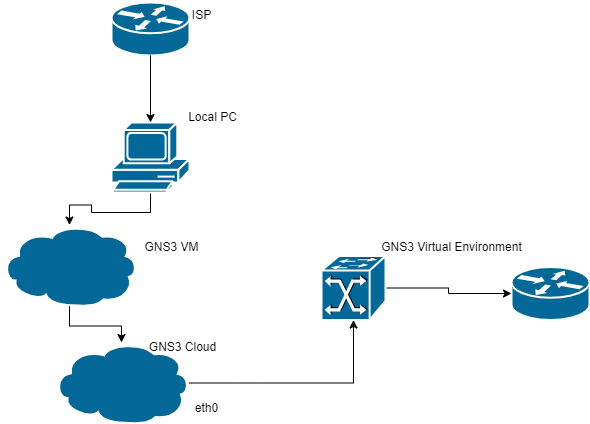
\includegraphics[width=0.7\textwidth]{graphics/diagram.drawio.png}
	\caption{\en{Local PC-GNS3VM-CISCO IOS Connection Architecture} }
\end{figure}









\section{\en{Connection Establishment} }


Όταν λοιπόν γίνει αυτή η παραμετροποίηση και τοπολογία θα πρέπει όλα αυτά τα διαφορετικά components να ανήκουν στο ίδιο τοπικό δίκτυο.
Η εικονική διεπαφή από την οποία θα περνάει όλη η κίνηση είτε μιλάμε για \en{REST} ειτε για \en{SSH} θα είναι η \en{eth0} στο \en{GNS3 VM}. Παρακάτω ένα 
\en{trace} στην εικόνα 4.5 που συλλέχτηκε αποδεικνύει ότι η σύνδεση πραγματοποιείται χωρίς προβλήματα.

\begin{figure}[htb]
	\centering
	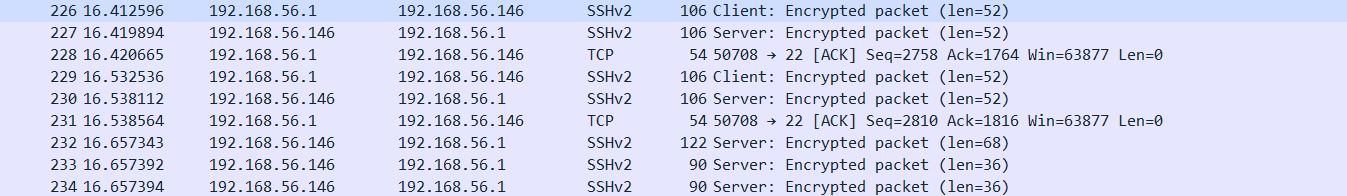
\includegraphics[width=0.7\textwidth]{graphics/ssh_connection.png}
	\caption{\en{SSH traffic} }
\end{figure}


Προκειμένου να γίνει η συλλογή του συγκεκριμένου \en{trace} χρησιμοποιήθηκε η παρακάτω εντολή:
\en{ tcpdump -i eth0 -v -w /home/gns3/test.pcap}
.Η συλλογή του \en{trace} έγινε με το πρωτόκολλο \en{SFTP}.


\begin{figure}[h]
	\centering
	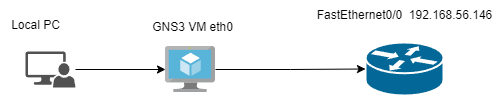
\includegraphics[width=0.7\textwidth]{graphics/jason1.png}
	\caption{\en{SSH traffic} }
\end{figure}

\FloatBarrier

\section{Σύνδεση με \en{Django Server} }

Ο \en{Django Server} τρέχει στον τοπικό υπολογιστή. Μπορεί να τρέξει σε οποιοδήποτε
μηχάνημα είναι \en{Linux} είτε \en{Windows} αρκεί να είναι στο τοπικό δίκτυο
είτε να υπάρχει κάποια συσκευή \en{layer2} η οποία να αναλάβει τη σύνδεση στο λεγόμενο
\en{data link layer}.

\section{Δομή της διαδικτυακής εφαρμογής \en{Django} }


\subsection{Τα αρχεία \en{urls.py}}
Αυτά τα αρχεία καθορίζουν τη δρομολόγηση \en{URL} της εφαρμογής. Οι διευθύνσεις \en{URL} που ταιριάζουν με
με τα μοτίβα \en{URL} που περιγράφονται στο αρχείο \en{urls.py}, αποστέλλονται στην αντίστοιχη
συνάρτηση στο αρχείο \en{views.py}. Η αντιστοίχιση γίνεται από πάνω προς τα κάτω στο αρχείο
\en{urls.py}. Ενώ το ακριβές ταίριασμα \en{URL} υλοποιήθηκε σε αυτό το έργο,
το \en{Django} επιτρέπει επίσης τη χρήση ταυτοποίησης κανονικών εκφράσεων. Στην εικόνα παρακάτω,
φαίνονται οι διευθύνσεις \en{URL} του \en{API} όπου κάθε διεύθυνση \en{URL} αντιστοιχεί στη συνάρτηση στο αρχείο
\en{api1/views.py} που καταλήγει στην εκτέλεση του σεναρίου.

\begin{figure}[htb]
	\centering
	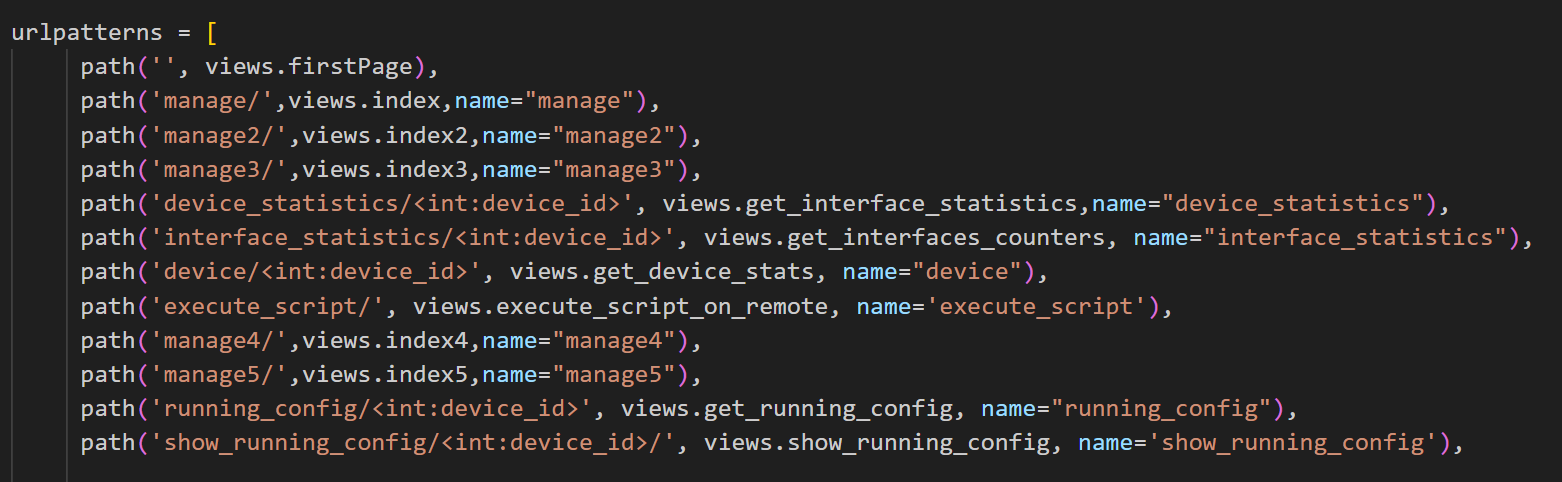
\includegraphics[width=0.9\textwidth]{graphics/urlpy.png}
	\caption{\en{url.py} }
\end{figure}

\subsection{Τα αρχεία \en{views.py}}

Οι συναρτήσεις σε ένα αρχείο \en{views.py} καλούνται όταν η δεδομένη διεύθυνση \en{URL} που αποστέλλεται από το
χρήστη ταιριάζει με το αντίστοιχο μοτίβο \en{URL} στο αρχείο \en{urls.py}. Παράμετροι που αποστέλλονται μέσω κλήσης
\en{HTTP} εισέρχονται στην αντίστοιχη συνάρτηση μέσω παραμέτρων ή σώματος αίτησης. Στο αρχείο \en{views.py} του \en{API}, η συνάρτηση εκτελεί το σενάριο
κώδικα με τις δεδομένες παραμέτρους εισόδου. Όταν τελειώσει η εκτέλεση του κώδικα δέσμης ενεργειών,
το αποτέλεσμα επιστρέφεται στη συνάρτηση \en{views} και μεταβιβάζεται ως πλαίσιο στο αντίστοιχο αρχείο \en{.html} για την εμφάνιση των αποτελεσμάτων στον χρήστη που εκτέλεσε το σενάριο.
Ένα παράδειγμα μιας συνάρτησης σε ένα αρχείο en{views.py} μπορείτε να δείτε στο σχήμα παρακάτω

\begin{figure}[htb]
	\centering
	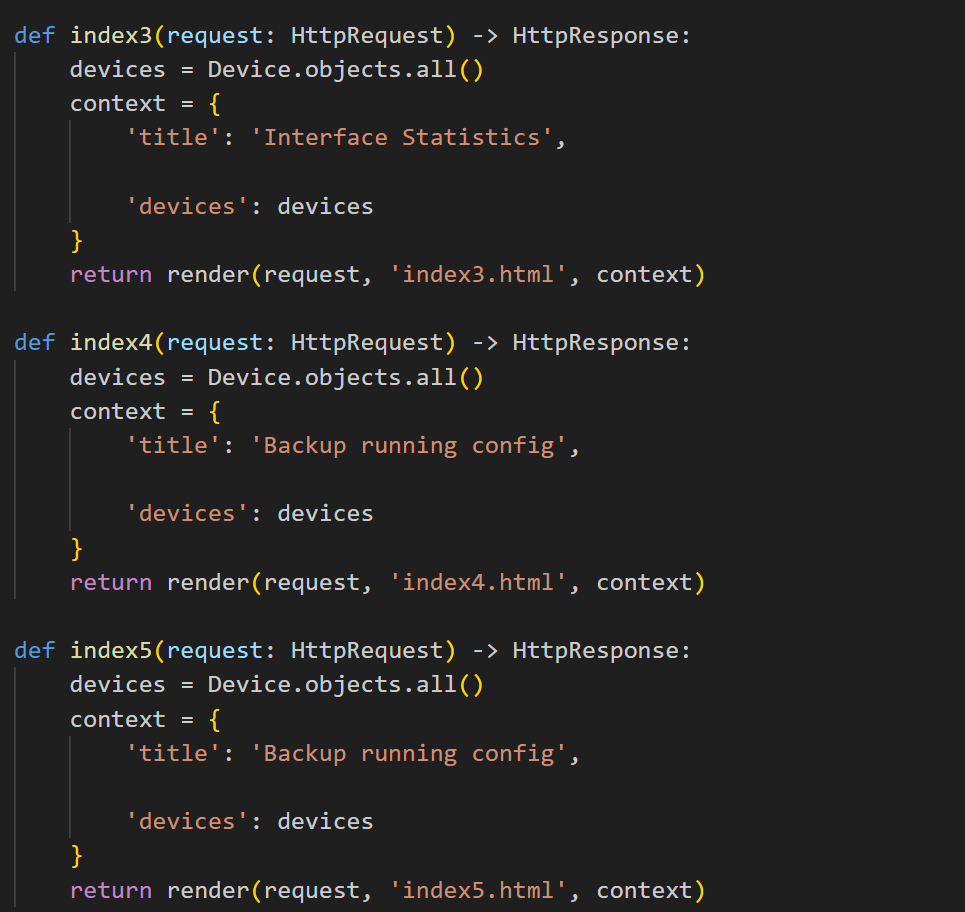
\includegraphics[width=0.9\textwidth]{graphics/viewspy.png}
	\caption{\en{views.py} }
\end{figure}

\subsection{Τα αρχεία \en{html template}}

Στη συνάρτηση \en{views.py}, το \en{Django} αποδίδει το αντίστοιχο πρότυπο \en{.html}
αρχείο με ένα συγκεκριμένο πλαίσιο. Το πλαίσιο είναι σε μορφή \en{JavaScript Object Notation (JSON)} και αποστέλλεται στο αρχείο \en{.html}. Τα δεδομένα στο πλαίσιο εμφανίζονται
στο \en{.html}, εάν το \en{.html} έχει παραμετροποιηθεί κατάλληλα. Ένα παράδειγμα \en{.html} με
τον συντακτικό κώδικα για τον τρόπο πρόσβασης στα δεδομένα του πλαισίου παρουσιάζεται στην εικόνα παρακάτω



\begin{figure}[htb]
	\centering
	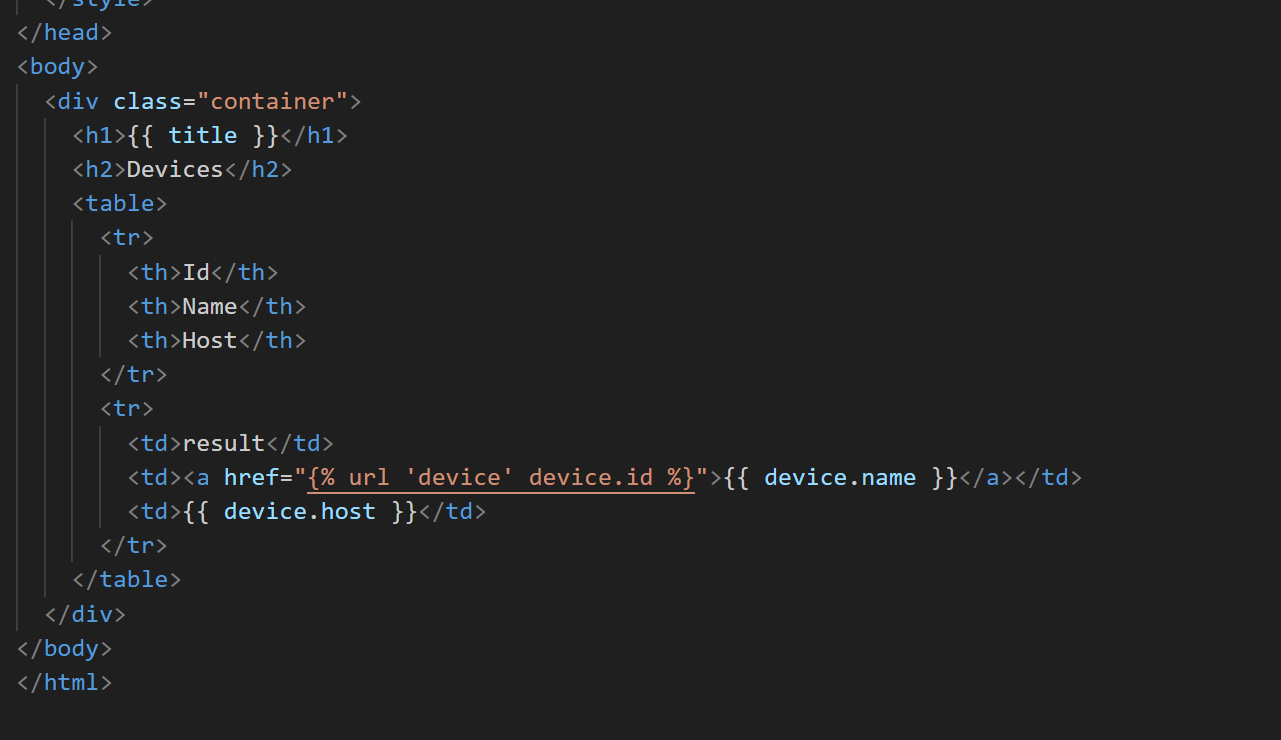
\includegraphics[width=0.9\textwidth]{graphics/html_template.png}
	\caption{Παράδειγμα \en{html} αρχείου }
\end{figure}